\documentclass[preprint]{aastex}
\let\captionbox\relax
\usepackage{geometry}                % See geometry.pdf to learn the layout options. There are lots.
\geometry{letterpaper}                   % ... or a4paper or a5paper or ... 
%\geometry{landscape}                % Activate for for rotated page geometry
%\usepackage[parfill]{parskip}    % Activate to begin paragraphs with an empty line rather than an indent
\usepackage{graphicx}
\usepackage{hyperref}
\usepackage{amssymb}
\usepackage{epstopdf}
\usepackage[justification=centering]{caption}
\DeclareGraphicsRule{.tif}{png}{.png}{`convert #1 `dirname #1`/`basename #1 .tif`.png}

\makeatletter
\let\@dates\relax
\makeatother

\citestyle{aa}

\title{Planetary Astrophysics: \\ Homework 1}
\author{Samuel Factor}
%\date{\today}           % Activate to display a given date or no date

\begin{document}
\maketitle

\section{Question 1}
Code for my model can be found at \url{https://github.com/sfxfactor/PlanetaryHW1}. I implemented an \texttt{Orbit} object which stores the orbital parameters and the masses of the two bodies. There are then two methods associated with an \texttt{Orbit} object, \texttt{calcCoord} which, given a time or array of times, calculates the $X$, $Y$, and $Z$ coordinates along with $r$ and the 3 anomaly angles $f$, $E$ and $M$. The second method, \texttt{calcObs} calculates the observables given a time or array of times. This method returns the projected seperation and position angle of the two bodies, the projected seperation and position angle of each body with respect to the center of mass, the radial velocity of both objects as well as the coordinates returned by \texttt{calcCoord}.

\section{Question 2}

Orbital parameters of HD 80606 b from the literature are presented in Table \ref{tab:orbparams} along with sources. A plot of stellar radial velocity (RV) versus time spanning August 1 to December 31, 2015 (JD 2457235.5 to 2457387.5) is shown in Figure \ref{fig:RV}. The maximum and minum RV's occur on the nights of October 16 and 18.

\begin{table}[h]
\begin{center}
    \caption{Orbital Parameters for HD 80606 b }\label{tab:orbparams} 
    \begin {tabular}{lcl}
    \tableline\tableline
    Parameter & Value & ref \\
    $a$ [AU] &  &  \\
    $e$ & & \\
    $i$ [deg] & & \\
    $\Omega$ [deg] & & \\
    $\omega$ [deg] & & \\
    $t_0$ [JD] & & \\
    $M_1$ [M$_\sun$] & & \\
    $M_2$ [M$_\mathrm{jup}$] & & \\
    \tableline
\end{tabular}
\end{center}
\end{table}

\begin{figure}[h]
\begin{center}
    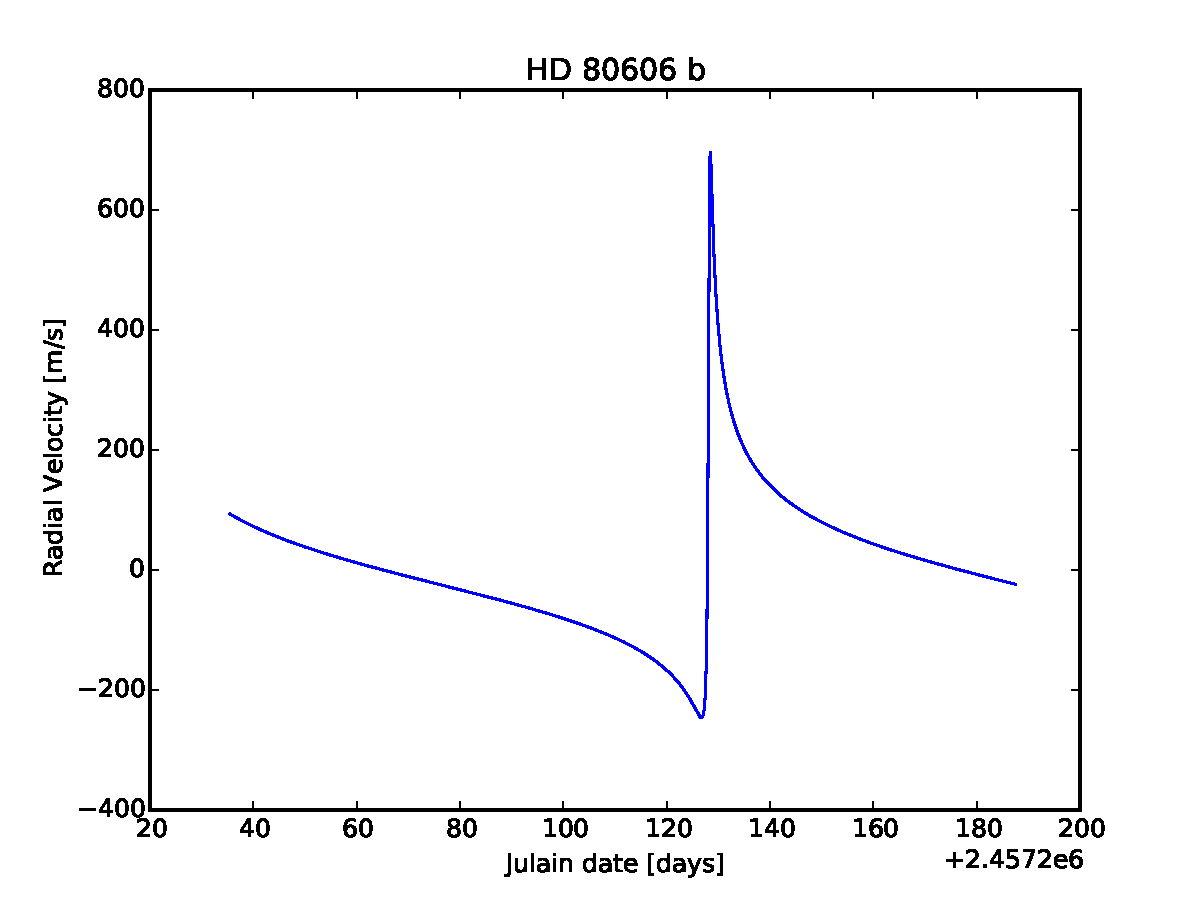
\includegraphics[width=\textwidth]{Q2.pdf}
    \caption{Radial velocity plot for HD 80606 b from August 1 to December 31, 2015}
    \label{fig:RV}
\end{center}
\end{figure}

\section{Question 3}

HD 80606 was observed by the Hipparcos satalite to have a paralax of ------ mas, corresponding to a distance of -----. As HD 80606 is a G5V we can approximate its radius as 1 $R_\sun$. The radius of the planet is $0.921\pm0.036$ $M_\mathrm{jup}$. With this information we can calculate the projected seperation of the planet and star which would result in a transit. 

\section{Question 4}



%\subsection{}

\end{document}  
